%%%%% SOME OPTIONS %%%%% 
\newcommand{\german}{false} % germanTrue or false --> Switch between german and english headers / titlepage
\newcommand{\coloredTitlePage}{true} % Switch between colored and BW titlepage
\newcommand{\company}{false}
\newcommand{\ECE}{true}
%%%%% Required Settings for the template %%%%%
\input{LaTeX/ECEconfig.sty}
\usepackage{hyperref}

\makeglossaries

\makeatletter
\newcommand{\myscope}[2] % #1 = name , #2 = rotation angle
{\draw[thick,rotate=#2] (#1) circle (12pt)
 (#1) ++(-0.35,-0.1) -- ++(0.3,0.3) --++(0,-0.3)-- ++(0.3,0.3) --++(0,-0.3);
}
\newcommand{\costumPicWidth}[0]{
0.8\textwidth
}

\newcommand{\costumPlotWidth}[0]{
\textwidth
}

%\addto\extrasngerman{\def\figureautorefname{Abbildung}}
%\addto\extrasngerman{\def\equationautorefname{Gleichung}}
%\addto\extrasngerman{\def\tableautorefname{Tabelle}}

\input{LaTeX/Einheiten}

\begin{document}
\input{LaTeX/frontmatter/glossaries}
%frontmatter inluding:
%titlepage, abstract, acknowledgments, declaration, toc, lof, lot
\frontmatter
\renewcommand{\thepage}{\Roman{page}}

\input{LaTeX/frontmatter/titlepage}

\tableofcontents
\printglossary
%mainmatter inluding: Parts, chapters, sections, appendicies
\mainmatter
%Hier die verschiedenn tex_Dokumente der Labore einfügen
\chapter{Balanbot Hardware Adaptions}
Due to lockdown restrictions and unavailable charging plugs, the existing battery of the Balanbot could not be used. Therefore, the Balanbot had to be converted to a 4S LiPo battery. The cable that supplies the motorshield also had to be changed. The battery can be fixed to two different variants. However, this also leads to different behavior of the balancing offer. In the next chapter, these two options are compared and a decision is made.

Furthermore, the new fixation of the cable can be seen in these pictures. Both the batteries and the cable are fixed with cable ties to the Balanbot.
\begin{figure}[H]
    \centering
    \includegraphics[width=0.8\textwidth]{Lab_report/pics/hardware_adapt/bat_lower_pos.jpg}
    \caption{Possible Battery position Nr. 1}
    \label{fig:lower_bat_pos}
\end{figure}

\begin{figure}[H]
    \centering
    \includegraphics[width=0.8\textwidth]{Lab_report/pics/hardware_adapt/bat_upper_pos.jpg}
    \caption{Possible Battery position Nr. 2 }
    \label{fig:upperlower_bat_pos}
\end{figure}

\begin{figure}[H]
    \centering
    \includegraphics[width=0.8\textwidth]{Lab_report/pics/hardware_adapt/cable.jpg}
    \caption{cable attachment}
    \label{fig:cable}
\end{figure}



\chapter{Model Building}
\section{Glossar}
For a better understanding of the explanations on the following pages, all used formula symbols have been summarized and explained here. Great care has been taken to assign each value to an unambiguous formula symbol.
\begin{figure}[H]
    \centering
    \includegraphics[width=0.4\textwidth]{Lab_report/pics/modelBuilding/300px-Cart-pendulum.svg.png}
    \caption{Sketch of the Balanbot}
    \label{fig:balanbot_sketch}
\end{figure}
% Please add the following required packages to your document preamble:
% \usepackage[table,xcdraw]{xcolor}
% If you use beamer only pass "xcolor=table" option, i.e. \documentclass[xcolor=table]{beamer}
\begin{table}[H]
\centering
\caption{Glossary }
\label{tab:glossary}
\begin{tabular}{|lx{1pt}l|l|}
\hline
\rowcolor[HTML]{C0C0C0} 
character      & description                                                                            & unit                     \\ \Xhline{1}
$x$            & Position of cart, may also be used as velocity: $\dot{x}$ and acceleration: $\ddot{x}$ & $m$,$^m/_s$, $^m/_{s^2}$ \\ \hline
$\Phi$         & Pendulums position                                                                     & degree                   \\ \hline
$m_{cart}$     & Mass of the cart                                                                       & kg                       \\ \hline
$m_{pendulum}$ & Mass of the pendulum                                                                   & kg                       \\ \hline
$\mu$          & Friction coefficient                                                                   & .                        \\ \hline
$I$            & Moment of inertia                                                                      & $^m/_{s^2}$               \\ \hline
$F$            & Force generated by the motors acting in the movement direction                         & N                        \\ \hline
$F_x$          & Force in horizontal direction acting between pendulum and cart                         & N                        \\ \hline
$F_y$          & Force in vertical direction acting between pendulum and cart                           & N                        \\ \hline
$F_r$          & Friction force acting against the movement direction of the cart                       & N                        \\ \hline
$g$            & Gravitational Constant                                                                 & $^m/_{s^2}$               \\ \hline
$l$            & Length of pendulum                                                                     & $m$                      \\ \hline
$x_G$           &Distance in x-direction of the pendulum to the center of gravity of the system         &$m$                        \\ \hline
$y_G$           &Distance in y-direction of the pendulum to the center of gravity of the system         &$m$                        \\ \hline
$b$            &Coefficient for F\textsubscript{r}                                                      & $\frac{kg}{s}$                      \\ \hline
\end{tabular}
\end{table}

\section{Model development}
The four base equations of the system have been derived from the sketch shown in \autoref{fig:forces}.

\begin{figure}[H]
    \centering
    \includegraphics[width=0.4\textwidth]{Lab_report/pics/modelBuilding/forces.png}
    \caption{Sketch of the Balanbot, forces included}
    \label{fig:forces}
\end{figure}

    \begin{align}    \label{eq: base 1 (a)}
        a = \ddot{x} = \frac{\sum F}{m_{cart}} = \frac{F-F_x-F_r}{m_{cart}}
    \end{align}

    \begin{align}    \label{eq: base 2 (alpha)}
            \ddot{\Phi} = \alpha = \frac{\sum T}{I} = \frac{F_x(cos(\Phi)-F_y sin(\Phi))}{I}
    \end{align}

    \begin{align}   \label{eq: base 3 (F_x)}
        F_x = m_{pendulum} \cdot \ddot{x_G} \notag\\
        x_G = x + l sin(\Phi)\notag \\
        \dot{x_G} = \dot{x} + l \dot{\Phi} cos(\Phi)\notag \\
        \ddot{x_G} = \ddot{x} - l \dot{\Phi} sin(\Phi) + l \ddot{\Phi} cos(\Phi)\notag \\ \cline{1-2}
        F_x = m_{pendulum}\cdot(\ddot{x} - l \dot{\Phi} sin(\Phi) + l \ddot{\Phi} cos(\Phi))
    \end{align}
 
    \begin{align}   \label{eq: base 4 (F_y)}
        F_y = m_{pendulum} \cdot (\ddot{y_G} + g)\notag \\
        y_G = l  cos(\Phi)\notag \\
        \dot{y_G} = -l  \dot{\Phi}  sin(\Phi)\notag \\
        \ddot{y_G} = -l \dot{\Phi}^2  cos(\Phi) - l \ddot{\Phi} sin(\Phi)\notag \\\cline{1-2}
        F_y = m_{pendulum} \cdot (g - l \dot{\Phi}^2  cos(\Phi) - l \ddot{\Phi} sin(\Phi))
    \end{align}
    After deriving the base equations from the system, the next goal is to merge the equations and receive final equations in the following form: $\ddot{x} = \dots$ and $\ddot{\Phi} = \dots$. The first final equation describes the acceleration of the system, the other one the angle of the pendulum. To receive this form, \autoref{eq: base 3 (F_x)} gets inserted into \autoref{eq: base 1 (a)}.
    
    \begin{align}\label{eq: final eq for x ddot}
        \ddot{x} \cdot m_{cart} = F-m_{pendulum}(\ddot{x}-l\dot{\Phi}^2 sin(\Phi)+l \ddot{\Phi} cos (\Phi))-\underbrace{b\dot{x}}_\text{F\textsubscript{r}})\notag \\
         \ddot{x} m_{cart} = F-m_{pendulum}\cdot\ddot{x}+m_{pendulum}l\dot{\Phi}^2 sin(\Phi)-m_{pendulum}l\ddot{\Phi}cos(\Phi)-b\dot{x}\notag \\
         \ddot{x}(m_{cart}+m_{pendulum})+b\dot{x}=F+m_{pendulum}l\dot{Phi}^2 sin(\Phi)-m_{pendulum}l\ddot{\Phi}cos(\Phi)\notag \\\notag \\\hline \notag \\
         \ddot{x} = \frac{F+m_{pendulum}l\dot{\Phi}^2 sin(\Phi)-m_{pendulum}l\ddot{\Phi}cos(\Phi)-b\dot{x}}{m_{cart}+m_{pendulum}}
    \end{align}
    \\
    To obtain $\ddot{\Phi} = \dots$, \autoref{eq: base 3 (F_x)} and \autoref{eq: base 4 (F_y)} get inserted into \autoref{eq: base 2 (alpha)}:
    \begin{align} \label{eq: final eq for Phi ddot}
        \ddot{\Phi} I = m_{pendulum} (\ddot{x} - l\dot{\Phi}^2 sin(\Phi) + l\ddot{\Phi} cos(\Phi))\cdot lcos(\Phi)-m_{pendulum}(g-l-\dot{\Phi}^2 cos(\Phi)-l\ddot{\Phi}sin(\Phi))\cdot l\sin(\Phi)\notag \\\notag\\
        \ddot{\Phi} I = m_{pendulum} l cos(\Phi) \ddot{x} \cancel{- m_{pendulum} l^2 cos(\Phi) sin(\Phi) \dot{\Phi}^2} + m_{pendulum} l^2 cos^2(\Phi) \ddot{\Phi} - m_{pendulum}g l sin(\Phi) \dots \notag\\ \dots \cancel{+m_{pendulum}l^2 sin(\Phi)cos(\Phi)\dot{\Phi}^2}+m_{pendulum}l^2 sin^2(\Phi)\ddot{\Phi}\notag \\\notag \\
        \ddot{\Phi} I = m_{pendulum} l cos(\Phi) \ddot{x} + m_{pendulum} l^2 \ddot{\Phi} (\underbrace{cos^2(\Phi)+sin^2(\Phi)}_\text{= 1})-m_{pendulum} g l sin(\Phi)\notag \\
         \ddot{\Phi} I + m_{pendulum}l^2\ddot{\Phi} = m l cos(\Phi)\ddot{x} + m_{pendulum} g l sin(\Phi)\notag \\\cline{1-2}\notag \\
         \ddot{\Phi} = \frac{m_{pendulum}\cdot lcos(\Phi)\ddot{x}+m_{pendulum}\cdot glsin(\Phi)}{I+m_{pendulum}\cdot l^2}
    \end{align}

\subsection{Consequence for the placement of the battery}
The first discussion point should revolve around what physically happens when the battery is placed lower, or higher on the balanbot. As the battery moves further from the axles center (note: the battery generates around xx\% of the balanbots mass), the moment of inertia increases too (\cite{enwiki:satz_von_steiner}). Also the center of gravity moves up the balanbot. 
\subsection{Model of the system}
\subsubsection{Cart}

\subsubsection{Pendulum}

\section{Analysis of the System}
\subsection{Linearization}



\subsection{Comparison of linear vs. non-linear System}

\subsection{System Analysis with Transfer Function}

Open loop response with no offset
Open loop response with initial condition $\Phi = 5^\circ$

\chapter{Controller Development}
\section{Proportional Gain}
In a first approach in controlling this system a proportional gain was installed. The gain will be used in further sections to find the parameters for a PID controller by using the Ziegler-Nichols method.

The simulation was taken with different values for gain. All of the results are plotten in \autoref{fig:prop_gain_non_linearized}
\begin{figure}[H]
    \centering
    \subfigure[$\text{gain }=1$]{\label{fig:prop_gain_non_linearized_g1}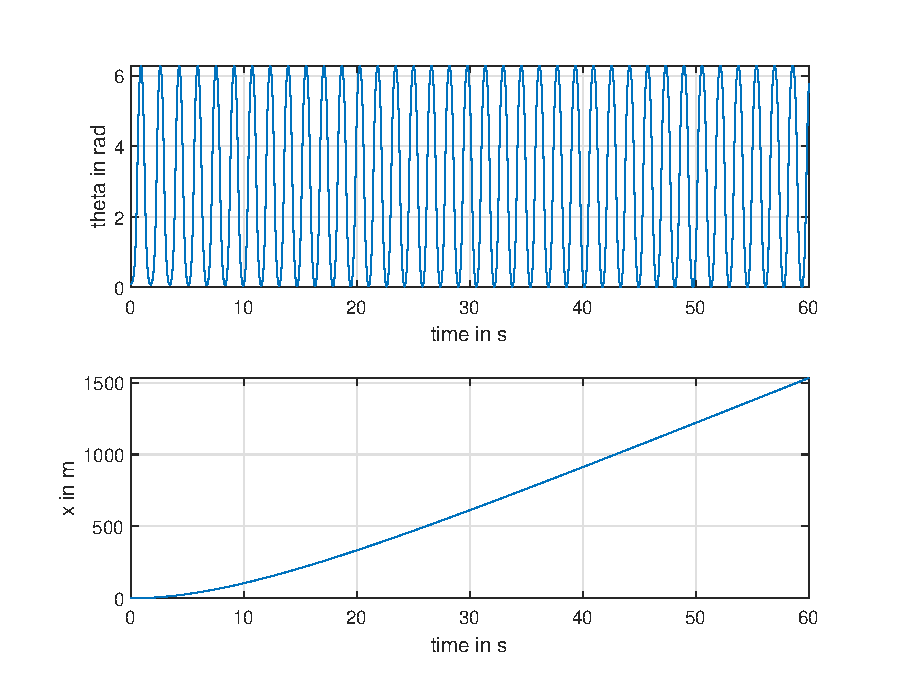
\includegraphics[width=0.49\textwidth]{Lab_report/pics/plots/non_linear_control_g1.eps}}
    \subfigure[$\text{gain }=5$]{\label{fig:prop_gain_non_linearized_g5}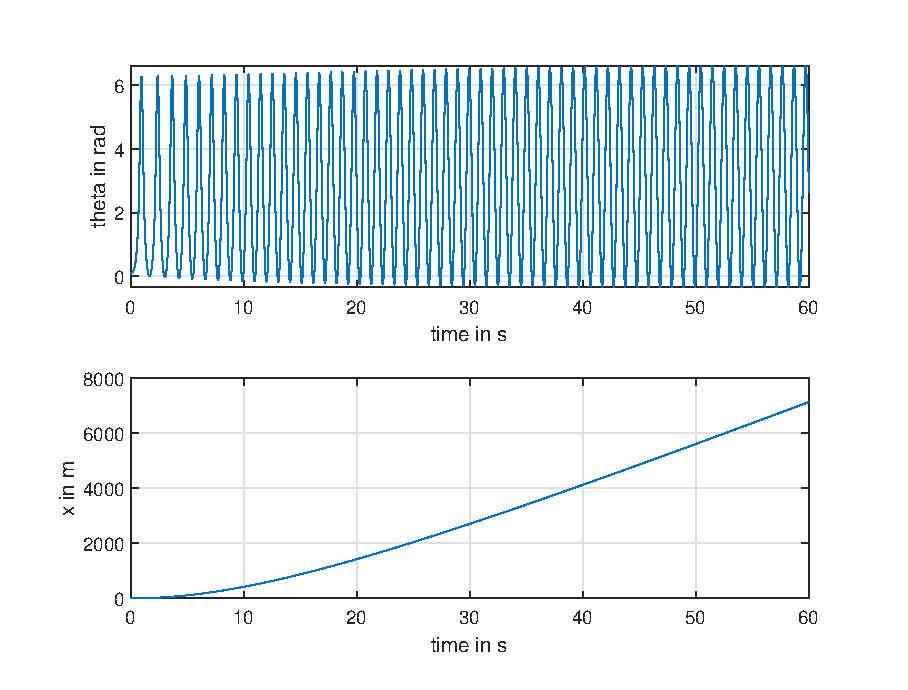
\includegraphics[width=0.49\textwidth]{Lab_report/pics/plots/non_linear_control_g5.eps}}
    \subfigure[$\text{gain }=10$]{\label{fig:prop_gain_non_linearized_g10}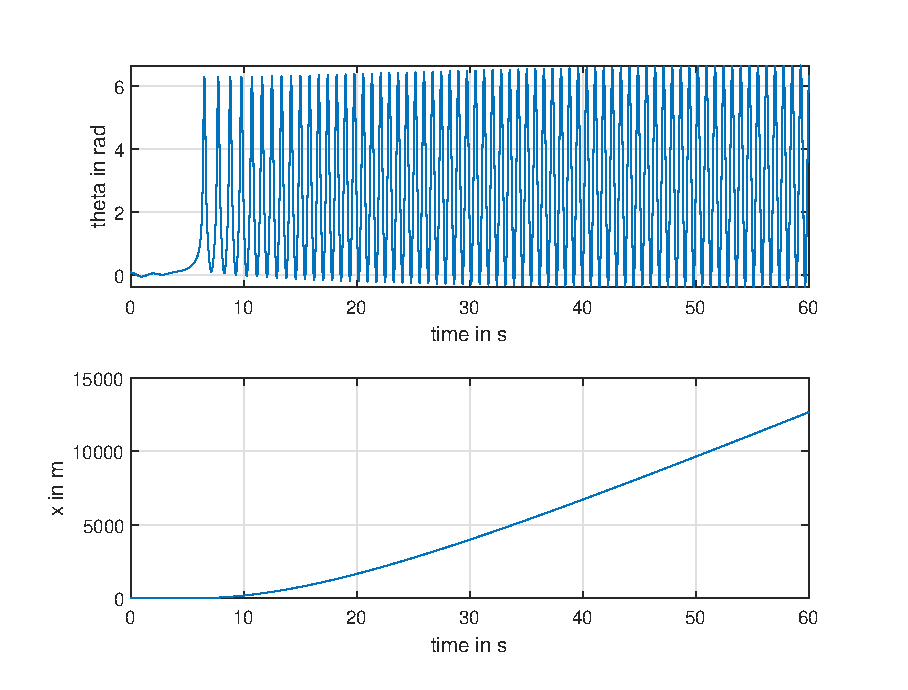
\includegraphics[width=0.49\textwidth]{Lab_report/pics/plots/non_linear_control_g10.eps}}
    \subfigure[$\text{gain }=15$]{\label{fig:prop_gain_non_linearized_g15}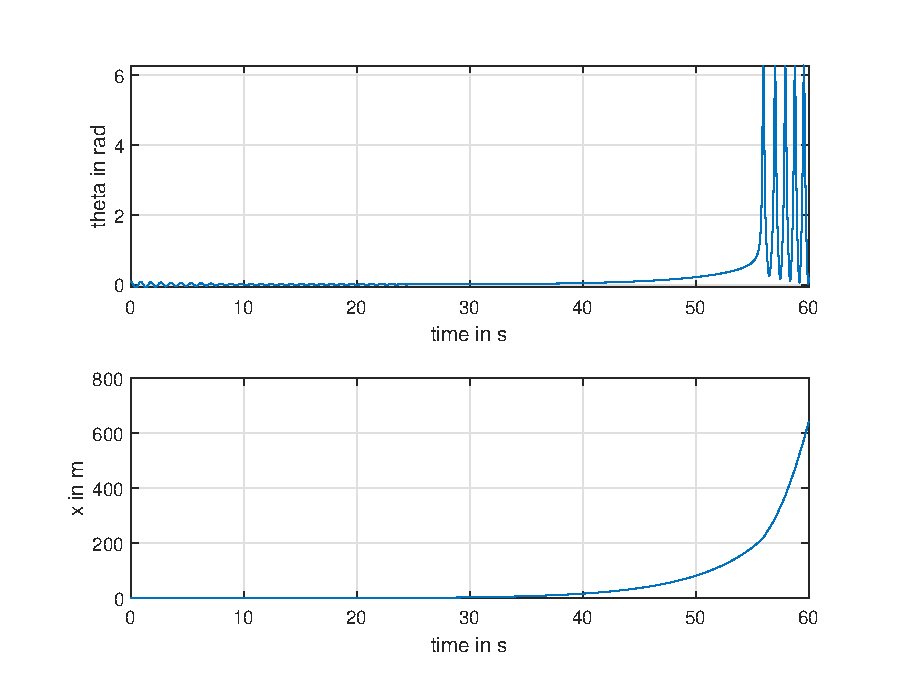
\includegraphics[width=0.49\textwidth]{Lab_report/pics/plots/non_linear_control_g15.eps}}
    \subfigure[$\text{gain }=20$]{\label{fig:prop_gain_non_linearized_g20}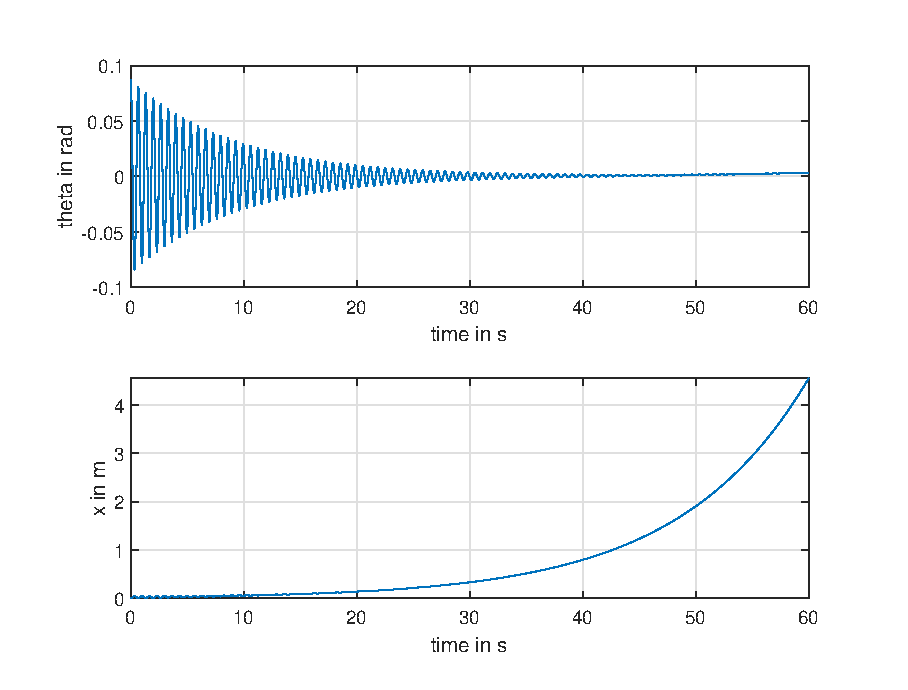
\includegraphics[width=0.49\textwidth]{Lab_report/pics/plots/non_linear_control_g20.eps}}
    \subfigure[$\text{gain }=22.5$]{\label{fig:prop_gain_non_linearized_g22_5}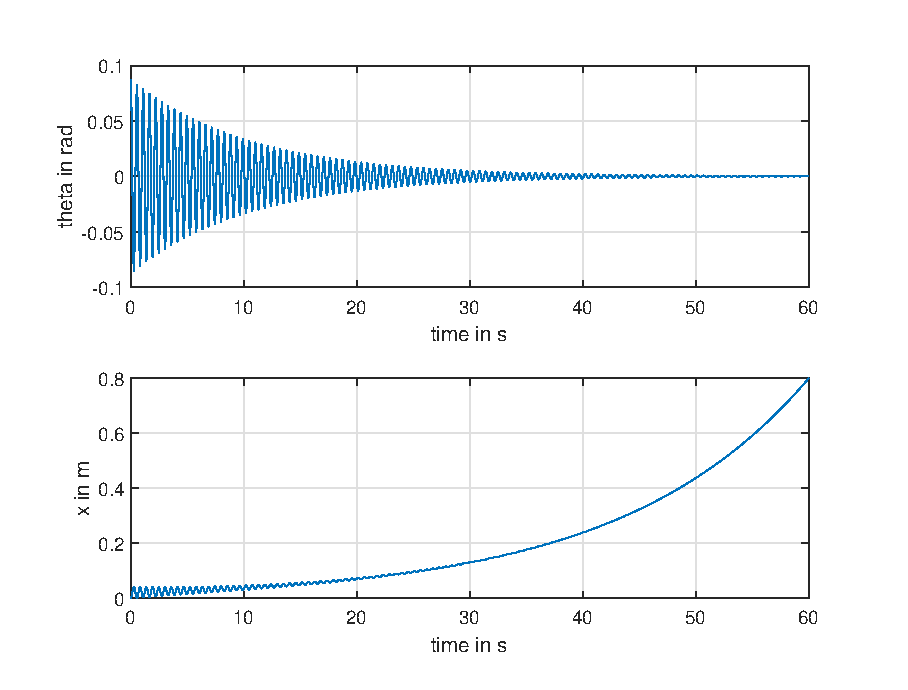
\includegraphics[width=0.49\textwidth]{Lab_report/pics/plots/non_linear_control_g22_5.eps}}
    \caption{simulation results of non linearized Model}
    \label{fig:prop_gain_non_linearized}
\end{figure}

% Please add the following required packages to your document preamble:
% \usepackage[table,xcdraw]{xcolor}
% If you use beamer only pass "xcolor=table" option, i.e. \documentclass[xcolor=table]{beamer}
\begin{table}[H]
\centering
\caption{oscillation periods and stable response, when simulation non-linearized systems with different $k_p$}
\label{tab:sim_res_non_linearized_kp}
\begin{tabular}{|l|l|l|}
\hline
\rowcolor[HTML]{C0C0C0} 
$k_p$ & $T_{osc} \text{in sec}$ & stable response (Y/N) \\ \hline
1     & $1.754$                 & N                     \\ \hline
5     & $1.390$                 & N                     \\ \hline
10    & $1.195$                 & N                     \\ \hline
15    & $1.118$                 & N                     \\ \hline
20    & $0.936$                 & N                     \\ \hline
22.5  & $0.870$                 & N                     \\ \hline
\end{tabular}
\end{table}

\chapter{Hardware Implementation}
\section{Task Clarification}
Until now a model was developed and with this model settings for a PID controller were found. To test these settings on the real BalanBot, a Simulink model which implements the hardware specific functions is needed. This includes reading the acceleration and gyroscope sensors, filtering and processing them and writing to the output registers. This ensures that the BalanBot also moves in a different direction with a negative output of the controller than with a positive output. 

\section{Detailed Code Commentary}
\subsection{Sensor Data Reading}
The IMU communicates with the Arduino via the I2C bus. This must be implemented in the Simulink design. The sensor values obtained from this must now be further ground via Matlab function blocks. To get more trustworthy data in the later course of the program, a Kalman filter was also used. However, this filter needs both the measured angle and the measured yaw rate for proper operation. Therefore these two values were calculated. 

\begin{figure}[H]
    \centering
    \includegraphics[width=1.1\textwidth]{Lab_report/pics/hardware_impl/gyro_read.PNG}
    \caption{Data reading Submodel}
    \label{fig:acc_gyro_read}
\end{figure}

\begin{lstlisting}[language=Matlab, caption=angle calculation]
function roll = fcn(i2c_sens_data)
    accX = double(i2c_sens_data(1));
    accY = double(i2c_sens_data(2));
    accZ = double(i2c_sens_data(3));
    roll = atan(accY / sqrt(accX * accX + accZ * accZ)) * 180/pi; 
end
\end{lstlisting}

\begin{lstlisting}[language=Matlab, caption=gyro rate calculation]
function [gyroXrate,gyroYrate,gyroZrate] = fcn(i2c_sens_data)
    gyroX = double(i2c_sens_data(5));
    gyroY = double(i2c_sens_data(6));
    gyroZ = double(i2c_sens_data(7));
    gyroXrate = gyroX/131;
    gyroYrate = gyroY/131;
    gyroZrate = gyroZ/131; 
end
\end{lstlisting}

\subsection{Data Processing}
In this submodel, the determined data is first filtered by a Kalman filter and then fed to the control algorithm. The data processing by means of this filter is described in more detail below.
\subsubsection{Kalman filter}
The principle of this filter is based on the estimation of the output quantity and the comparison of the measured output quantity. The difference of these two quantities is then weighted with the Kalman gain and used to correct the estimated output value. In our case the code for this estimation and correction algorithm is already finished and only a small test and proof of concept will be shown here. 

\subsubsection{Controller}
To control the BalanBot, a PID controller was implemented after the Kalman filter.
\begin{figure}[H]
    \centering
    \includegraphics[width=\textwidth]{Lab_report/pics/hardware_impl/motor-control.PNG}
    \caption{Model of the Motor Control}
    \label{fig:motor control model}
\end{figure}

The PID-Controller Submodel looks as can be seen in \autoref{fig:pid_model}.
\begin{figure}[H]
    \centering
    \includegraphics[width=\textwidth]{Lab_report/pics/hardware_impl/PID.PNG}
    \caption{Model of the PID Controller}
    \label{fig:pid_model}
\end{figure}
To 
The angle limit was also implemented into the PID-Controller Submodel. If the angle of the BalanBot is bigger than $40^\circ$ or smaller than $-40^\circ$ , the output (= motor speed) gets set to 0RPM.
\newline\\\\
\textbf{Adjusting of the PID-Controller gains}\\
The settings of the PID controller had already been estimated by using the Simulink model beforehand. However, when testing these settings on the real BalanBot, the PID-Controller could not stabilize the BalanBot.\\\\
To obtain some reasonable PID-Controller parameter values, all gains have been initially set to zero. Then, the proportional gain was estimated at first. To get rid of the steady-state-error, a integral gain was also estimated and implemented. However, the BalanBot reacted way too aggressive to faster errors, hence a derivative gain was estimated and implemented.\\\\
The fine tuning of the controller was done in the following order:
\begin{itemize}
    \item Adjusting the proportional gain until the outcome was somewhat nearly satisfactory
    \item Adjusting the integral gain in combination with the proportional gain so the BalanBot would react fast enough but not too strong to errors
    \item Adjusting the derivative gain to smooth the aggressiveness of the controller
\end{itemize}

The final PID-Controller gains can be seen in \autoref{fig:pid_model}.
\subsection{Motor Control}


\chapter{Tests and Validation}
A video of the working BalanBot can be viewed by scanning the QR-code below or simply following this link: \url{https://www.youtube.com/watch?v=ocpmd9iVG38}
\begin{figure}[H]
    \centering
    \includegraphics[width=0.25\textwidth]{Lab_report/pics/testvalid/frame.png}
    \caption{QR-Code linking a youtube-video of the working BalanBot}
    \label{fig:balanbot_qe}
\end{figure}

\newpage
\chapter{Signaturen}
    Fertig gestellt am \today \\
    \begin{figure}[H]
        \centering
        \includegraphics{LaTeX/pics/signature_grebien.png}
    	\caption{Signatur: Grebien Alexander}
    	\label{pic:signatur_grebien}
    \end{figure}
        
\listoffigures
\listoftables
\bibliographystyle{ieeetr}
\bibliography{meine_Zitatsbibliothek.bib}
\end{document}
